\chapter{Методика использования}

В данной главе будет изложена методика применения разработанного SDK, представлены области применения, описаны основные шаги использования SDK и их результаты.

\section{Области применения}

Разработанный инструментальный пакет предназначен для создания инструментов статического анализа динамически формируемых строковых выражений. Решения, созданные с помощью описанного SDK, могут использоваться для работы с проектами, активно использующими динамически формируемые строковые выражения, и применяться в следующих областях.

\begin{itemize}
    \item Реинжиниринг программного обеспечения.
    \item Поддержка встроенных языков в средах разработки.
    \item Оценка качества и сложности кода.
\end{itemize}

Общим для всех этих областей является то, что для решения многих задач необходимо структурное представление динамически формируемого кода. При этом анализируемые языки могут быть различными и процесс их анализа часто тесно связан с анализом внешнего языка.

Отметим, что встроенные языки используются всё менее активно в молодых проектах и системах. На смену им приходят более надёжные способы композиции языков и метапрограммирования. Например LINQ или ORM-технологии. Однако это не всегда так. Использование строковых выражений для взаимодействия с базами данных и генерации WEB-страниц в приложениях на PHP всё ещё широко распространено. Это необходимо учитывать при поддержке встроенных языков в средах разработки. Для каких-то языков на первый план выходят возможности по изучению и модификации уже созданного кода, а для каких-то --- возможность быстро и удобно создавать новый код. Во втором случае могут возникнуть дополнительные требования к скорости работы инструмента, так как подразумевается выполнение некоторых операций ``на лету'', что может послужить ограничением на использование SDK, так как многие механизмы, реализованные в нём, не предусматривают возможности уменьшения точности в пользу увеличения быстродействия.

Оценка качества и сложности  кода часто может выполняться в рамках комплекса задач по реинжинирингу системы, однако может быть и самостоятельной задачей, например, при оценке сложности работ по поддержке и сопровождению информационной системы.


\section{Способы применения}

Детали применения SDK могут варьироваться в зависимости от решаемых задач и контекста использования. Например, механизм построения регулярной аппроксимации может быть реализован независимо в рамках внешнего инструмента. Однако основной сценарий использования аналогичен использованию инструментариев для разработки компиляторов. Последовательность шагов, представленная ниже может быть изменена в зависимости от особенностей задачи.

\begin{itemize}
    \item Создание грамматики обрабатываемого языка. Грамматика может быть создана на основе документации соответствующего языка или переиспользована готовая, что оправданно, например, при создании анализатора для динамического SQL, когда внешний и встроенный языки совпадают.
    \item Генерация синтаксического анализатора по созданной грамматике. Для этого используется генератор синтаксических анализаторов, присутствующий в SDK. Результатом работы генератора является файл с исходным кодом на языке программирования F\#, который должен быть включён в разрабатываемый код. Файл содержит описание типов для лексических единиц, управляющие таблицы анализатора и функцию, которая по конечному автомату над алфавитом токенов анализируемого языка построит SPPF, содержащий деревья вывода всех корректных цепочек.
    \item Создание лексической спецификации обрабатываемого языка. Спецификация может быть извлечена из документации или заимствована из других проектов. При обработке динамически формируемого SQL возможно переиспользовать спецификацию, созданную для основного языка, которым также является SQL. При этом необходимо обратить внимание на то, что типы лексических единиц определяются на основе созданного на предыдущих шагах синтаксического анализатора.
    \item Генерация лексера по созданной спецификации. Для этого применяется генератор лексических анализаторов, входящий в состав SDK. В результате его применения получается файл с исходным кодом на языке F\#, который должен быть подключён к разрабатываемому решению. 
    \item Реализация механизма построения регулярной аппроксимации, результатом которого является функция, строящая конечный автомат над алфавитом символов. Данный механизм может быть реализован либо на основе предоставляемого в рамках SDK, либо независимо. В первом случае от разработчика требуется построить обобщённый CFG для внешнего языка. Во втором случае необходимо только гарантировать правильность возвращаемого конечного автомата. Второй подход может быть использован, например, при наличии реализованного механизма протягивания констант для внешнего языка. Это позволит создать возможно менее точное, но, скорее всего, более быстрое построение аппроксимации. Такой подход применим при автоматизированном реинжиниринге, когда ручная доработка кода является обязательным шагом и абсолютная точность автоматической обработки не требуется. Ещё одна возможная область применения второго подхода --- это поддержка встроенных языков в средах разработки. Здесь также часто не требуется высокая точность для подсказок пользователю, однако производительность крайне важна. Поэтому иногда приходится жертвовать точностью анализа для достижения нужной скорости работы.
    \item Реализация работы с SPPF. Синтаксический анализатор возвращает SPPF --- конечное представление леса разбора всех корректных цепочек из аппроксимации. Дальнейшая работа с ним может строиться по двум основным сценариям.
    \begin{itemize}
        \item Непосредственная обработка SPPF. В этом случае все вычисления происходят над SPPF без извлечения отдельных деревьев. Это позволит ускорить обработку результатов разбора, так как количество деревьев может быть бесконечным, а SPPF является конечной структурой данных. Однако существует несколько проблем, связанных с таким подходом. Во-первых, требуется создание новых процедур обработки, так как классические, как правило, ориентированы на работу с деревьями. Во-вторых, могут возникнуть трудности при выполнении некоторых анализов, вызванные тем, что в SPPF хранятся ``бесконечные'' деревья. Например, необходимо вычислить максимальную глубину вложенности конструкции \verb|if|, являющуюся одной из стандартных метрик сложности кода. SPPF может содержать 
циклы и может оказаться так, что конструкция \verb|if| встречается в цикле таким образом, что потенциальная глубина вложенности может быть бесконечной. Такая ситуация не является стандартной при 
обработке деревьев разбора и её надо отслеживать отдельно.
        \item Извлечение отдельных деревьев из SPPF и их обработка. Данный подход может оказаться удобным, если уже существуют процедуры обработки синтаксических деревьев для языка, который оказался встроенным. Это помогает избежать затрат на создание новой функциональности. Такое может произойти при работе с динамическим SQL. В этом случае для работы с деревом разбора внешнего языка и деревьями, извлечёнными из SPPF, можно использовать одни и те же процедуры, так как языки идентичны.

Недостатком данного подхода является то, что конечность числа деревьев не гарантирована. Это значит, что не удастся обработать все деревья. Стоит отметить, что даже в случае конечности числа деревьев, перебор и обработка всех деревьев разбора может потребовать значительных ресурсов.
    \end{itemize}
    \item Реализация механизмов сбора, обработки и отображения информации, такой как сообщения об ошибках или любой другой, полученной в процессе анализа. Необходимо для предоставления пользователю информации, ожидаемой в рамках решаемой задачи.
\end{itemize}

На рисунке~\ref{fig:activMethod} изображён один из возможных сценариев использования SDK. Особенностью является цикличность процесса, характерная, например для реинжиниринга программного обеспечения.

\begin{figure}[h!]
\begin{center}
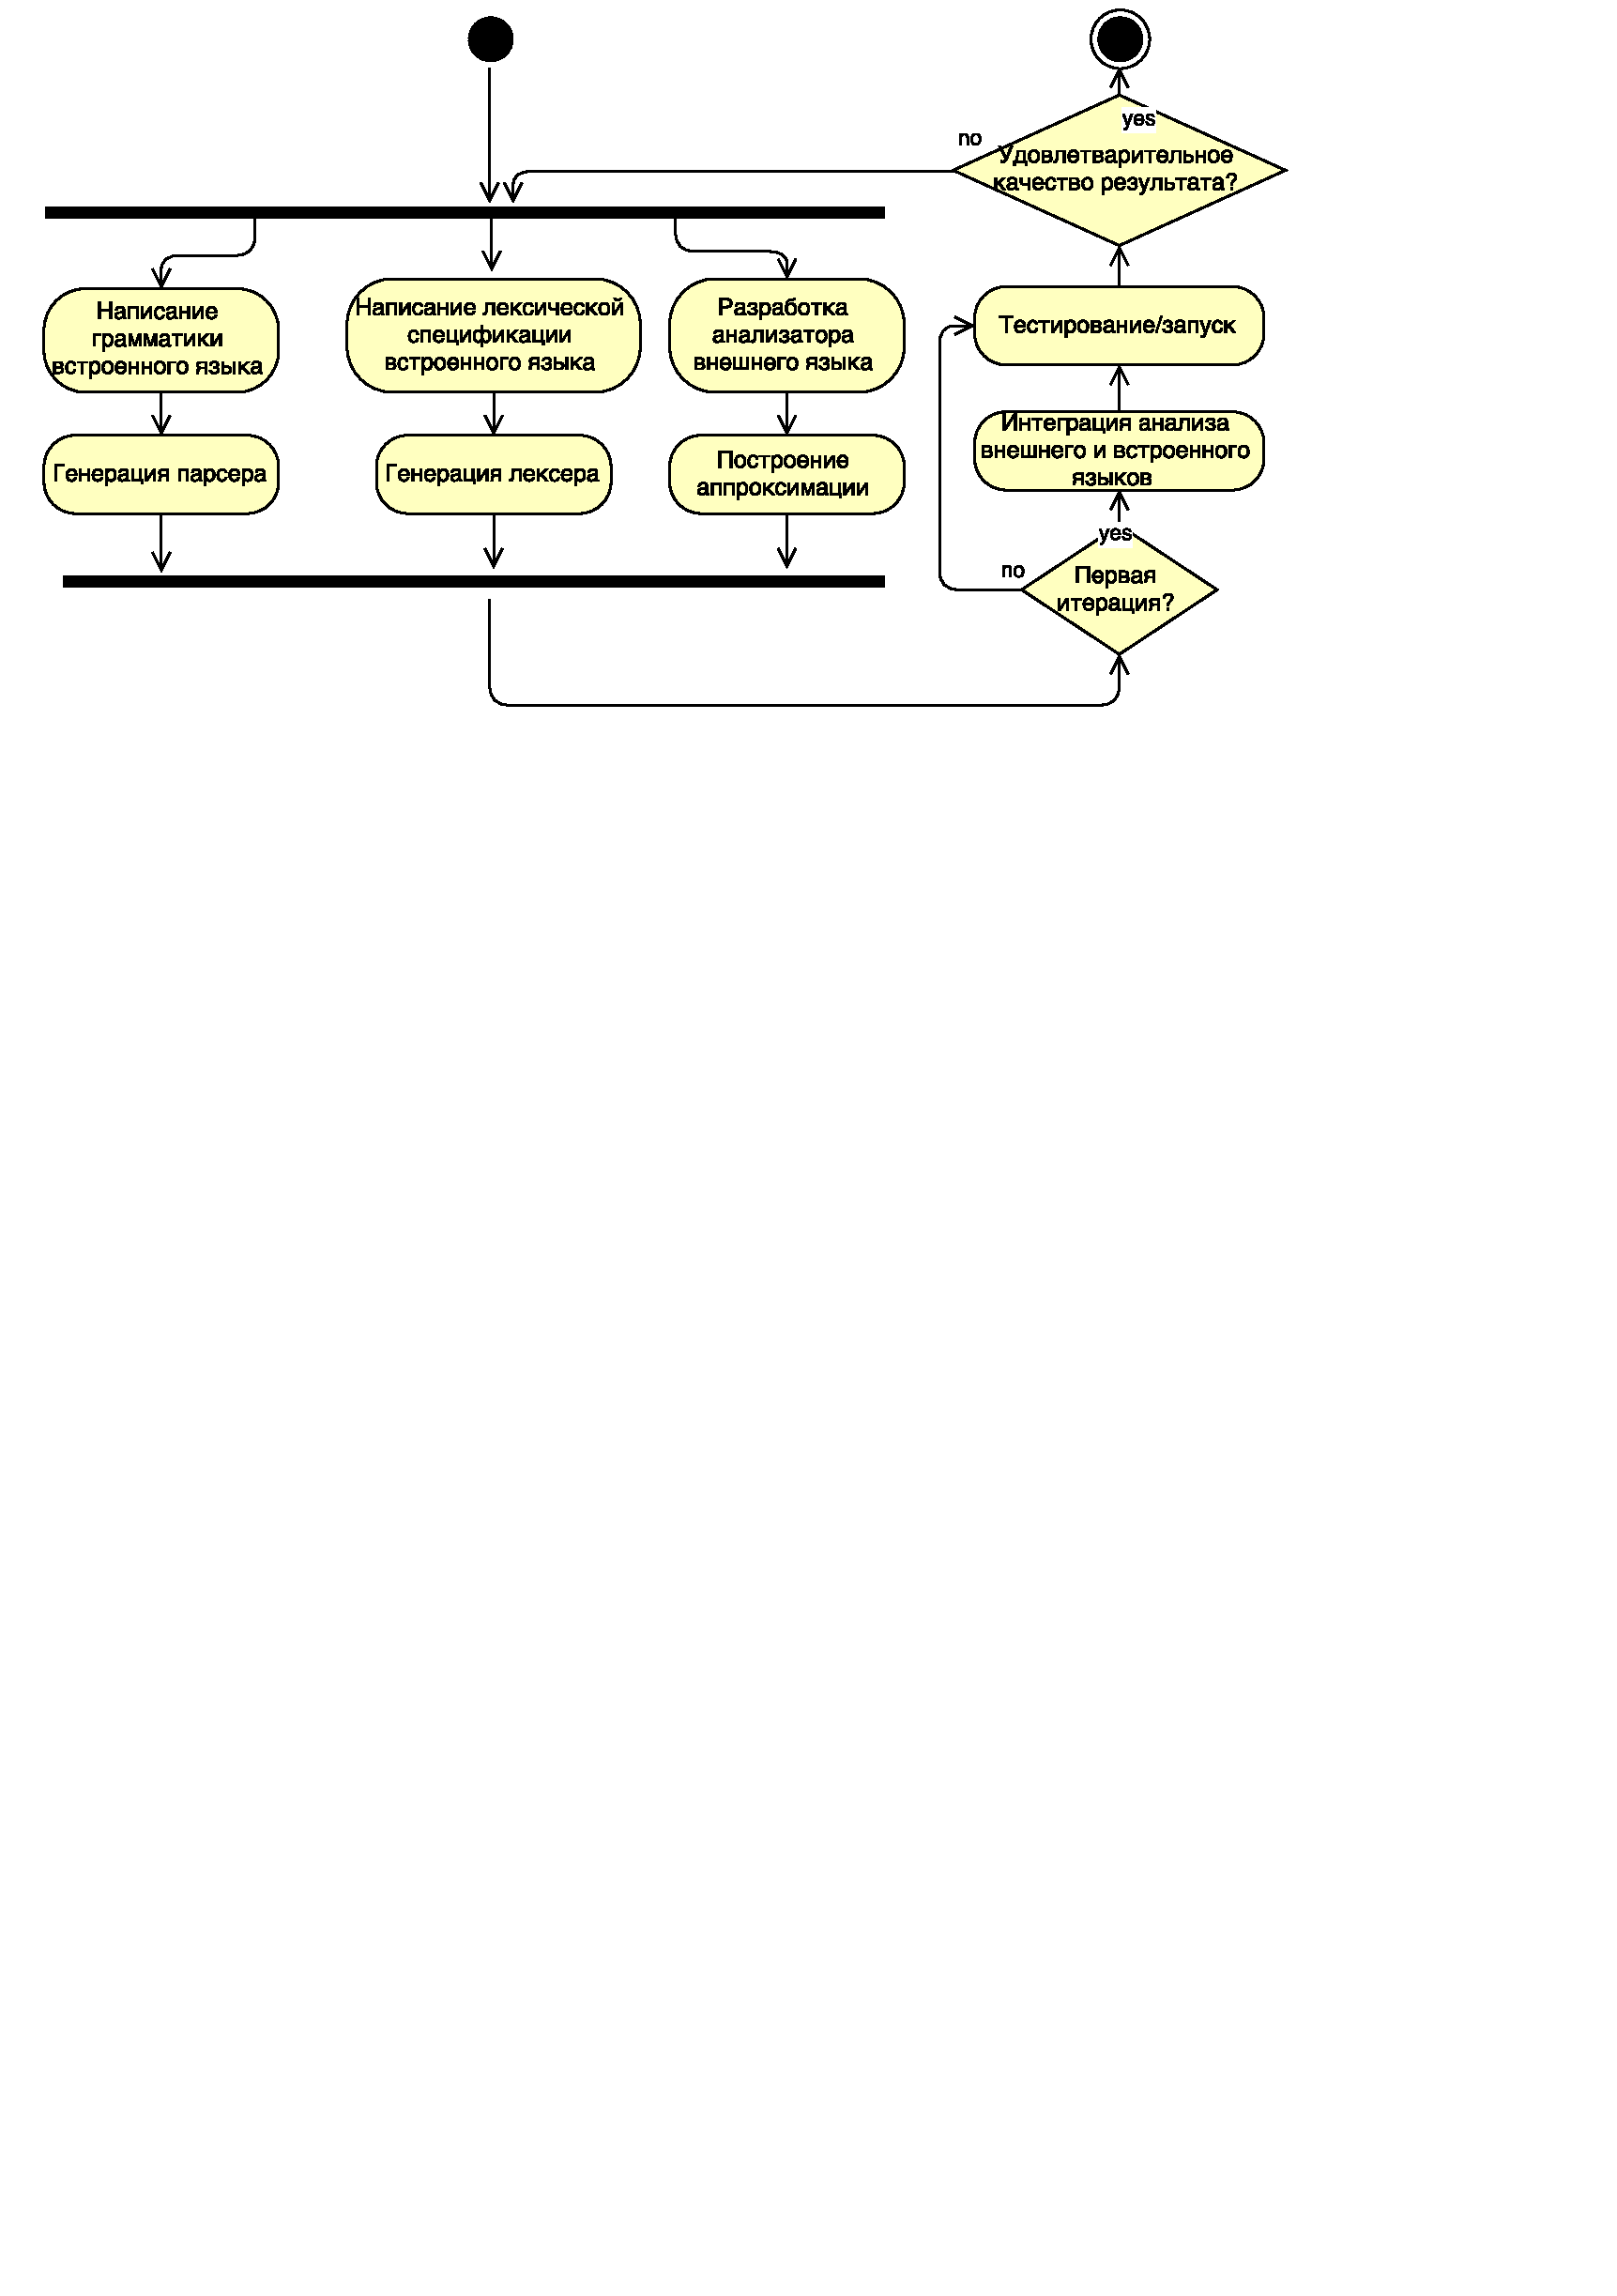
\includegraphics[width=0.9\textwidth]{pics/ActivMethodology}
\caption{Один из возможных вариантов использования SDK в проектах по реинжинирингу}
\label{fig:activMethod} 
\end{center}
\end{figure}

Встраивание анализа строковых выражений в последовательность обработки кода всей системы зависит от решаемых задач. Первыми шагами идут действия, необходимые для того, чтобы получить входные данные для анализа. Для этого необходимо провести лексический и синтаксический анализ внешнего языка, построить граф потока управления. После этого возможно построение аппроксимации и дальнейший анализ встроенных языков. Параллельно с этим может проводиться дальнейшая обработка внешнего языка. Степень параллельности зависит от независимости решаемых задач. Например, некоторые метрики сложности для основного кода и для динамически формируемого можно считать независимо и выводить отдельно. С другой стороны, может возникнуть необходимость вычислить некую комплексную метрику, учитывающую параметры и внешнего и динамически формируемого кода, что приведёт к необходимости синхронизации.

\clearpage
